% !TEX root = ../../../main.tex

\toggletrue{image}
\toggletrue{imagehover}
\chapterimage{time}
\chapterimagetitle{TIME}
\chapterimageurl{https://xkcd.com/1190/}
\chapterimagehover{The end.}

\chapter{Laufzeit von Suchalgorithmen}
\label{chapter-laufzeit-suchalgorithmen}

In \autoref{chapter-suchalgorithmen} (\nameref{chapter-suchalgorithmen}) wurde das Suchproblem durch zwei unterschiedliche Algorithmen gelöst. Welcher Algorithmus löst das Problem besser? Es gibt verschiedene Kriterien, um diese Frage zu beantworten:

\begin{itemize}
	\item Wie elegant ist der Pseudocode?
	\item Wie hoch ist der Programmieraufwand für einen Algorithmus?
	\item Wie viel Speicherplatz benötigt der Algorithmus?
	\item Wie lange dauert die Ausführung des Algorithmus?
	\item $\dots$
\end{itemize}

In der Informatik konzentrieren wir uns meistens auf die Dauer der Ausführung eines Algorithmus. Wir möchten in diesem Kapitel also die \textbf{Ausführungsdauer} der beiden \textbf{Suchalgorithmen} bestimmen und damit die beiden Suchalgorithmen miteinander vergleichen. Die Lernziele lauten:

\newcommand{\laufzeitSuchalgorithmenLernziele}{
\protect\begin{todolist}
\item Sie definieren den Begriff Laufzeit und erklären, warum wir diese Definition so gewählt hat.
\item Sie bestimmten die Laufzeit für einen Algorithmus mit einer gegebenen Eingabe.
\item Sie erklären, was wir unter der asymptotischen Laufzeit eines Algorithmus versteht.
\item Sie erklären die drei Varianten, die es für die Bestimmung der asymptotischen Laufzeit gibt.
\item Sie skizzieren die asymptotischen Laufzeiten in einem (kartesischen) Koordinatensystem.
\item Sie bestimmten für einen Algorithmus die asymptotische Worst-Case-Laufzeit.
\item Sie notieren für ein sortiertes Array den dazugehörigen binären Suchbaum.
\end{todolist}
} 

\lernziel{\autoref{chapter-laufzeit-suchalgorithmen}, \nameref{chapter-laufzeit-suchalgorithmen}}{\protect\laufzeitSuchalgorithmenLernziele}

\laufzeitSuchalgorithmenLernziele

\section{Wie messen wir die Ausführungsdauer eines Algorithmus?}

Wir könnten einen Algorithmus in eine Programmiersprache überführen, das Programm ausführen und die Zeit in Millisekunden stoppen, die der Algorithmus für die Verarbeitung der Eingabe benötigt. Besitzt ein Problem zwei unterschiedliche Algorithmen, dann führen wir für dieselbe Eingabe die beiden Algorithmen aus und vergleichen die Zeitdauer. Diese Methodik wäre möglich, beinhaltet jedoch ein paar offene Fragen:

\begin{itemize}
	\item Ein Computer kann dasselbe Programm unterschiedlich schnell ausführen. Ist die Ausführungsdauer in Millisekunden sinnvoll?
	\item Es gibt auch Unterschiede bei den Programmiersprachen. Es gibt \say{langsamere} und \say{schnellere} Programmiersprachen. Unterschiedliche Programmiersprachen könnten beim Vergleich zu unterschiedlichen Ergebnissen führen. Wie berücksichtigen wir dies?
\end{itemize}

Die Informatik hat deshalb nach einer Methode gesucht, um Algorithmen fair miteinander vergleichen zu können. Die Messung der \textbf{Ausführungsdauer} muss dabei \textbf{unabhängig} von einem Computer sein, der das Programm ausführt.

\begin{definition}[Laufzeit]
Die Laufzeit eines Algorithmus gibt an, wie viele \textbf{Elementaroperationen} ein Algorithmus benötigt, um die \textbf{Eingabe für ein Problem} zu bearbeiten.
\end{definition}

Damit wir die Definition besser verstehen, klären wir zunächst was eine Elementaroperation ist.

\subsection{Was ist eine Elementaroperation?}

Typischerweise besteht ein Algorithmus aus mehreren Elementaroperationen. Wir haben bereits folgende Elementaroperationen gesehen:

\begin{itemize}
	\item Zuweisungen ($\gets$)
	\item Vergleiche (z.B. $\leq$ oder $=$) in einer \lstinline[language=pseudocode]{if}-Anweisung
	\item arithmetische Operationen (Addition, Subtraktion, etc.)
\end{itemize}

Für die Bestimmung der Laufzeit wählen wir nun eine \textbf{charakteristische Elementaroperation} aus und zählen, wie oft die Elementaroperation ausgeführt wird. Was die charakteristische Elementaroperation ist, hängt von der Problemstellung und den Algorithmen ab.

\begin{example}
	Beim Suchproblem ist ein Array von Zahlen und eine gesuchte Zahl \lstinline[language=pseudocode]{k} gegeben. Sowohl die lineare, als auch die binäre Suche lösen das Problem, in dem wiederholt ein Vergleich zwischen der gesuchten Zahl und den Zahlen aus dem Array durchgeführt wird. Es liegt nahe, den \textbf{Vergleich zweier Zahlen} als \textbf{charakteristische Elementaroperation} zu wählen.
\end{example}

\subsection{Beispiele für Laufzeiten}

Wir betrachten das Array \lstinline{[2, 12, 27, 42, 66, 101, 1024]} und untersuchen die Laufzeiten für die lineare und binäre Suche für unterschiedliche, gesuchte Zahlen \lstinline[language=pseudocode]{k}.

\begin{example}[\texttt{k = 27}]
	Wir führen die lineare Suche mit dem gegebenen Array durch. \autoref{lst-algo-lin-suche-bsp-1} zeigt den Pseudocode. Wir zählen, wie oft der Algorithmus den Vergleich in Code-Zeile $4$ ausführt.
	\begin{lstlisting}[language={pseudocode}, caption={Lineare Suche für $n = 7$ und \texttt{k = 27}.}, label={lst-algo-lin-suche-bsp-1}]
input: A = [2, 12, 27, 42, 66, 101, 1024], k = 27
i $\gets$ 0
loop as long as i < 7 {
 if <@  \colorbox{lightgray}{A[i] = 27} @> then {
  output: Suche erfolgreich
  stop
 }
 Erhöhe i um 1
}
output: Suche erfolglos
\end{lstlisting}

Wir führen drei Vergleiche durch, bis die Suche stoppt. \autoref{table-lin-search-laufzeit-bsp-1} visualisiert das Resultat. Die Laufzeit für dieses Beispiel beträgt somit \textbf{drei Vergleiche}.
\end{example}

\begin{table}[htb]
\centering
\begin{minipage}{0.45\textwidth}
\centering
\begin{tabular}{|c|c|c|c|c|c|c|}
\hline
$0$ & $1$ & $2$ & $3$ & $4$ & $5$ & $6$ \\ \hline
$2$ & $12$ & $27$ & $42$ & $66$ & $101$ & $1024$ \\ \hline
$\diamond$ & $\diamond$ & \checkmark & & & & \\ \hline
\end{tabular}
\caption{$3$ Vergleiche: Index $0$, Index $1$ und Index $2$. Die Suche ist erfolgreich.}
\label{table-lin-search-laufzeit-bsp-1}
\end{minipage}
\hfill
\begin{minipage}{0.45\textwidth}
\centering
\begin{tabular}{|c|c|c|c|c|c|c|}
\hline
$0$ & $1$ & $2$ & $3$ & $4$ & $5$ & $6$ \\ \hline
$2$ & $12$ & $27$ & $42$ & $66$ & $101$ & $1024$ \\ \hline
$\diamond$ & $\diamond$ & $\diamond$ & $\diamond$ & $\diamond$ & $\diamond$ & \checkmark \\ \hline
\end{tabular}
\caption{$7$ Vergleiche: Die gesuchte Zahl befindet sich ganz am Ende.}
\label{table-lin-search-laufzeit-bsp-2}
\end{minipage}
\end{table}

\begin{example}[\texttt{k = 1024}]
	Wir führen die lineare Suche mit dem gegebenen Array erneut durch und zählen wieder die Anzahl der Vergleiche. Wir erhalten eine Laufzeit von \textbf{sieben} Vergleichen, wie \autoref{table-lin-search-laufzeit-bsp-2} zeigt.
\end{example}


\begin{example}[\texttt{k = 2}]
	Wir führen die binäre Suche mit dem gegebenen Array durch. \autoref{lst-algo-bin-suche-bsp-1} zeigt den Pseudocode. Wir zählen, wie oft der Algorithmus einen Vergleich ausführen muss (Code-Zeile 7, Code-Zeile 11 oder Code-Zeile 14).
	
\begin{lstlisting}[language=pseudocode, caption={Binäre Suche für $n = 7$.}, label={lst-algo-bin-suche-bsp-1}]
input: A = [2, 12, 27, 42, 66, 101, 1024], k = 2
indexLinks $\gets$ 0
indexRechts $\gets$ 6
loop as long as indexLinks $\leq$ indexRechts {
 indexMitte $\gets$ (indexLinks + indexRechts) // 2
 kandidat $\gets$ A[indexMitte]
 if <@  \colorbox{lightgray}{kandidat = 2} @> then {
  output: Suche erfolgreich
  stop
 }
 elseif <@  \colorbox{lightgray}{kandidat > 2} @> then {
  indexRechts $\gets$ indexMitte - 1
 }
 elseif <@  \colorbox{lightgray}{kandidat < 2} @> then {
  indexLinks $\gets$ indexMitte + 1
 }
}
output: Suche erfolglos
\end{lstlisting}

Wir benötigen drei Vergleiche, bis wir das Ergebnis ermittelt haben. \autoref{table-bin-search-laufzeit-bsp-1} visualisiert die Vergleiche.

\begin{table}[htb]
\centering
\begin{tabular}{|c|c|c|c|c|c|c|}
\hline
$0$ & $1$ & $2$ & $3$ & $4$ & $5$ & $6$ \\ \hline
$2$ & $12$ & $27$ & $42$ & $66$ & $101$ & $1024$ \\ \hline
\circled{3} & \circled{2} & & \circled{1} & & & \\ \hline
\end{tabular}
\caption{Es sind $3$ Vergleiche notwendig. Wir beginnen bei Index $3$.}
\label{table-bin-search-laufzeit-bsp-1}
\end{table}

Wir haben also hier eine Laufzeit von \textbf{drei Vergleichen}.

\end{example}

\subsection{Aufgaben}

\begin{enumerate}
\item Bestimmen Sie die Laufzeit für die lineare Suche für \lstinline[language=pseudocode]{k = 25} und dem Array \\ \lstinline[language=pseudocode]{A = [4, 8, 16, 20, 25, 35, 41, 56, 96, 97]}.

\fillwithgrid	{0.25in}

\item Bestimmen Sie die Laufzeit für die binäre Suche für \lstinline[language=pseudocode]{k = 25} und dem Array \\ \lstinline[language=pseudocode]{A = [4, 8, 16, 20, 25, 35, 41, 56, 96, 97]}.

\fillwithgrid	{0.25in}

\item Bestimmen Sie die Laufzeit für die lineare Suche für \lstinline[language=pseudocode]{k = 8} und dem Array \\ \lstinline[language=pseudocode]{A = [4, 8, 16, 20, 25, 35, 41, 56, 96, 97]}.

\fillwithgrid	{0.25in}

\item Bestimmen Sie die Laufzeit für die binäre Suche für \lstinline[language=pseudocode]{k = 8} und dem Array \\ \lstinline[language=pseudocode]{A = [4, 8, 16, 20, 25, 35, 41, 56, 96, 97]}.

\fillwithgrid	{0.25in}

\end{enumerate}

\section{Asymptotische Laufzeit}

Bei der Laufzeitanalyse von Algorithmen sind wir daran interessiert, wie sich ein Algorithmus verhält, wenn die Eingabe sehr gross wird. Wir gehen sogar noch weiter und möchten die \textbf{Laufzeit in Abhängigkeit von der Eingabegrösse} ermitteln.

\begin{definition}[Asymptotische Laufzeit]
	Kleine Eingabegrössen (z.B. $n = 100$) sind uninteressant. Wir interessieren uns für die Laufzeit bei sehr grossen Eingaben. Wir möchten die Laufzeit als \textbf{Funktion der Eingabe} darstellen. Diese Laufzeit wird asymptotische Laufzeit genannt und mit $T(n)$ bezeichnet.
\end{definition}

Bei den beiden Suchalgorithmen möchten wir somit die Laufzeit analysieren, falls die Anzahl der Zahlen sehr gross ist. Dabei unterscheiden wir typischerweise drei Varianten für die Angabe der asymptotischen Laufzeit:

\begin{itemize}
	\item \textbf{Best-Case} (dt. bester Fall): Wie lange benötigt ein Algorithmus bei einer idealen Eingabe? Die Laufzeit $T_{\text{BC}}(n)$ gibt an, wie lange der Algorithmus \textbf{mindestens} braucht für die Lösung eines Problems.
	\item \textbf{Average-Case} (dt. durchschnittlicher Fall): Die Berechnung der Laufzeit erfolgt im Sinne der Wahrscheinlichkeitsrechnung. Es wird eine erwartete Laufzeit $T_{\text{AC}}(n)$ berechnet, wobei die Wahrscheinlichkeit der verschiedenen Eingaben bekannt sein sollte.
	\item \textbf{Worst-Case} (dt. schlechtester Fall): Wie lange benötigt ein Algorithmus \textbf{maximal} für die Lösung eines Problems? Bei welcher Eingabe wird diese maximale Laufzeit $T_{\text{WC}}(n)$ erreicht?
\end{itemize}

Im Gebiet der Algorithmen sind wir daran interessiert, für einen Algorithmus eine Garantie bezüglich der Laufzeit anzugeben. Deshalb bestimmen wir oft die Laufzeit im schlechtesten Fall, das heisst $T_{\text{WC}}(n)$. Wir bestimmen in den nächsten beiden Abschnitten nun die asymptotische Laufzeit an einem konkreten Beispiel.

\section{Asymptotische Laufzeit für die lineare Suche}

Wir betrachten nun die lineare Suche und gehen stets davon aus, dass die gesuchte Zahl $k$ im Array $A$ vorhanden ist. Das Array besitzt $n$ Zahlen. Wir werden die Laufzeiten für die drei Varianten bestimmen. Wir erinnern uns daran, dass wir mit der Laufzeit die \textbf{Anzahl der Vergleiche} angeben.

\begin{itemize}
	\item Im \textbf{besten Fall} befindet sich die gesuchte Zahl im Array an der allerersten Position (Index $0$). Wir müssen in diesem Fall also exakt einen Vergleich durchführen, und zwar \textbf{unabhängig} von der Länge des Arrays. Wir erhalten die asymptotische Laufzeit $T_{\text{BC}}^{\text{lin}}(n) = 1$.
		\item Der \textbf{durchschnittliche Fall} lässt sich bei der linearen Suche über Wahrscheinlichkeiten berechnen. Wir erhalten $T_{\text{AC}}^{\text{lin}}(n) = \frac{n + 1}{2}$ Vergleiche.
	\item Im \textbf{schlechtesten Fall}  befindet sich die gesuchte Zahl am Ende des Arrays (Index $n-1$). In diesem Fall müssen wir $n$ Vergleiche durchführen. Wir erhalten: $T_{\text{WC}}^{\text{lin}}(n) = n$.
\end{itemize}

Die Resultate sind in \autoref{table-asymp-laufzeit-lin-search} zusammengefasst.

\begin{table}[htb]
\centering
\begin{tabular}{|c|c|c|c|}
\hline
Algorithmus & Best-Case & Average-Case & Worst-Case \\ \hline
Lineare Suche & $1$ & $\frac{n+1}{2}$ & $n$ \\ \hline
\end{tabular}
\caption{Asymptotische Laufzeiten für die lineare Suche mit $n$ Elementen.}
\label{table-asymp-laufzeit-lin-search}
\end{table}

Wir können die Funktionen in einem (kartesischen) Koordinatensystem (\say{x-y-Diagramm}) zeichnen. Auf der \say{x-Achse} tragen wir die Anzahl der Zahlen ein, das heisst $n$. Die \say{y-Achse} misst die Anzahl der Vergleiche. \autoref{figure-asymp-laufzeiten-lin-suche-plot} zeigt die Funktionen. Die Laufzeit für den Worst-Case der linearen Suche ist eine lineare Funktion ($T_{\text{WC}}^{\text{lin}}(n) = n$). Daher auch der Name des Suchalgorithmus.

\begin{figure}[htb]
	\centering
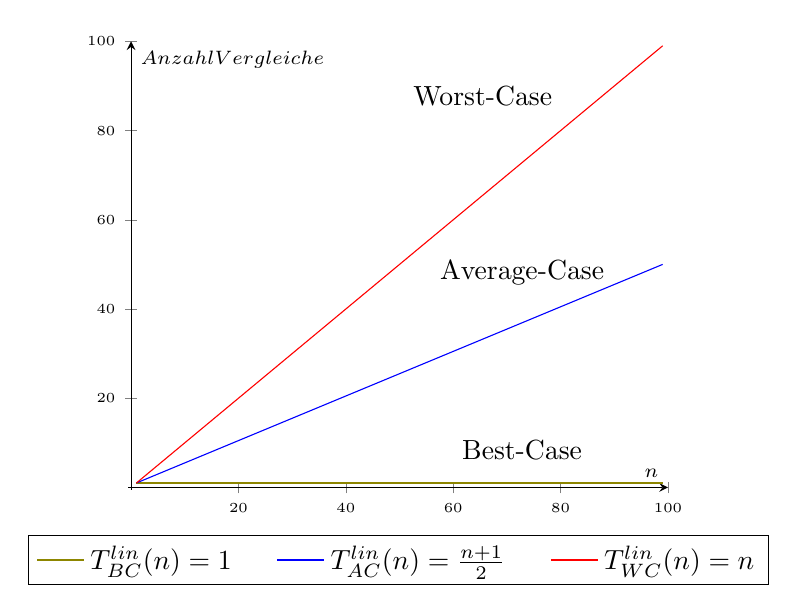
\begin{tikzpicture}
  \begin{axis}[axis lines=middle, xmin=-0.5, xmax=100, ymin=-0.5, ymax=100, xlabel=$\scriptstyle n$, ylabel=$\scriptstyle \text{Anzahl Vergleiche}$, tick label style={font=\tiny}, legend style={at={(0.5,-0.1)},anchor=north, /tikz/every even column/.append style={column sep=0.5cm}}, legend columns=-1]
    \addplot+[no marks, olive, domain=1:99, samples=99] {1};
    \addlegendentry{$T_{\text{BC}}^{\text{lin}}(n) = 1$}
    \addplot+[no marks, blue, domain=1:99, samples=99] {(x+1)/2};
    \addlegendentry{$T_{\text{AC}}^{\text{lin}}(n) = \frac{n+1}{2}$}
    \addplot+[no marks, red, domain=1:99, samples=99] {x};
    \addlegendentry{$T_{\text{WC}}^{\text{lin}}(n) = n$}
  \end{axis}
  \node at (4.5,5) {Worst-Case};
  \node at (5,2.75) {Average-Case};
  \node at (5,0.5) {Best-Case};
\end{tikzpicture}
\caption{Asymptotische Laufzeiten für die lineare Suche.}
\label{figure-asymp-laufzeiten-lin-suche-plot}
\end{figure}

\subsection{*Herleitung Average-Case}

Für die Berechnung des durchschnittlichen Falls müssen wir die erwartete Laufzeit berechnen. Dazu benötigen wir Kenntnisse der Stochastik (Wahrscheinlichkeitsrechnung), um den Erwartungswert der Laufzeit zu berechnen (erwartete Laufzeit). Wir zeigen dies hier am Beispiel der linearen Suche für den Average-Case.

Es ist ein Array mit $n$ \textbf{verschiedenen} Zahlen gegeben. Sei $E_i$ das Ereignis, dass die gesuchte Zahl $k$ im Array mit dem Index $i$ gespeichert ist. Es gibt somit $n-1$ Ereignisse, von $E_0$ bis und mit $E_{n-1}$. Wir erhalten somit für ein Ereignis $E_i$ die Wahrscheinlichkeit:
\begin{align*}
	P(E_i) = \frac{\text{Anzahl Zahlen mit } A[ i ]=k}{\text{Anzahl aller Zahlen}} = \frac{1}{n}
\end{align*}
Wir definieren nun die Zufallsvariable $X$, welche für jedes Ereignis misst, wie viele Vergleiche notwendig sind, bis wir die Zahl finden. Wir erhalten:
\begin{align*}
	X(E_0) &= 1 \\
	X(E_1) &= 2 \\
	X(E_2) &= 3 \\
	&\vdots\\
	X(E_{n-1}) & = n
\end{align*}
Nochmal umgangssprachlich: mit $X(E_2) = 3$ ist gemeint, dass beim Eintreffen des Ereignis $E_2$ (sprich die gesuchte Zahl ist im Array mit dem Index $2$ gespeichert), wir $3$ Vergleiche brauchen, bis wir die Zahl finden. Allgemein können wir also $X(E_{i}) = i+1$ verwenden. Nun können wir den Erwartungswert berechnen, das heisst die erwartete Laufzeit.
\begin{DispWithArrows*}[wrap-lines]
\mathbb{E}[X] 
&= X(E_0)\cdot P(E_0) + X(E_1)\cdot P(E_1) + \cdots + X(E_{n-1})\cdot P(E_{n-1}) \Arrow[i]{Summenzeichen verwenden} \\ 
&= \sum\limits_{i=0}^{n-1} X(E_i) \cdot P(E_i) \Arrow[i]{Wahrscheinlichkeit einsetzen} \\ 
&= \sum\limits_{i=0}^{n-1} X(E_i) \cdot \frac{1}{n} \Arrow[i]{Wert der Zufallsvariable einsetzen} \\
&= \frac{1}{n} \cdot \sum\limits_{i=0}^{n-1} (i+1) = \frac{1}{n} \cdot \sum\limits_{i=0}^{n-1} i + \frac{1}{n} \cdot \sum\limits_{i=0}^{n-1} 1 \Arrow[i, xoffset=1cm]{\say{Kleiner Gauss}} \\
& = \frac{1}{n} \cdot \frac{(n-1)\cdot((n-1)+1)}{2} + \frac{1}{n} \cdot n = \frac{(n-1)}{2} + 1 = \frac{n+1}{2}
\end{DispWithArrows*}

\section{Asymptotische Laufzeit für die binäre Suche}

Die Analyse der Laufzeiten ist für die binäre Suche nicht ganz so einfach, wie bei der linearen Suche. Es ist auf den ersten Blick nicht klar, wie oft ein Vergleich im Algorithmus aus \autoref{lst-algo-bin-suche} für eine gegebene Zahl $k$ durchgeführt werden muss. Vor der mathematischen Analyse lohnt es sich, die Suchstrategie der binären Suche zu visualisieren.

\begin{example}
Wir betrachten das Array \lstinline[language=pseudocode]{[2, 12, 27, 42, 66, 101, 1024]} und versuchen die Vergleiche, die während der binären Suche durchgeführt werden können in einem Baum darzustellen. Wir erhalten \autoref{binary-search-tree-example-1}.

\begin{figure}[htb]
	\centering
\begin{tikzpicture}[every node/.style={minimum size=0.75cm, inner sep=0pt}, level/.style={sibling distance=4.5cm/#1}, edge from parent/.style={draw, -latex}]
\node [circle, draw] (v0) {$42$}
	child {
		node [circle, draw] (v1) {$12$}
		child {
			node [circle, draw] (v2) {$2$}
		}
		child {
			node [circle, draw] (v3) {$27$}
		}
   	}
	child {
		node [circle, draw] (v4) {$101$}
		child {
			node [circle, draw] (v5) {$66$}
		}
		child {
			node [circle, draw] (v6) {\small $1024$}
		}
	};
\node[right=of v0, font=\bfseries] (l1) {Level 1};
\node[right=of v4, font=\bfseries] (l2) {Level 2};
\node[right=of v6, font=\bfseries] (l3) {Level 3};
\end{tikzpicture}
\caption{Der binäre Suchbaum für \lstinline{[2, 12, 27, 42, 66, 101, 1024]}.}
\label{binary-search-tree-example-1}
\end{figure}
\end{example}

Eine binäre Suche nach einer Zahl \lstinline[language=pseudocode]{k} beginnt immer im Level 1 und endet bei einer Zahl im untersten Level. Die Darstellung aus \autoref{binary-search-tree-example-1} ist ein binärer Suchbaum. 

\begin{definition}[Binärer Suchbaum]
Ein binärer Suchbaum besteht aus gerichteten Kanten (\say{Linien mit Pfeil}) und Knoten (\say{Kreise}) mit den gesuchten Zahlen darin. Bäume \say{wachsen} in der Informatik \say{auf dem Kopf}. Deshalb nennen wir den \say{obersten} Knoten \textbf{Wurzel}. Die \say{untersten} Knoten nennen wir \textbf{Blätter}. Wir teilen den binären Suchbaum in unterschiedliche Ebenen ein. Wir nennen eine Ebene \textbf{Level} und jeder Knoten in einem Level hat den gleichen Abstand zur Wurzel. Bei einem binären Suchbaum gibt es pro Knoten maximal \textbf{zwei} nachfolgende Knoten. Der \textbf{linke Knoten} besitzt immer eine Zahl, die \textbf{kleiner} ist als die Zahl im vorherigen Knoten. Der \textbf{rechte Knoten} besitzt immer eine Zahl, die \textbf{grösser} ist als die Zahl im vorherigen Knoten.
\end{definition}

\subsection{Was hat ein binärer Suchbaum mit der binären Suche zu tun?}

Wenn wir mithilfe des binären Suchbaums nach einer Zahl \lstinline[language=pseudocode]{k} suchen möchten, dann beginnen wir bei der Wurzel. Wir vergleichen die gesuchte Zahl mit der Zahl im Knoten. Ist die Zahl identisch, dann ist die Suche erfolgreich und wir stoppen. Ist die gesuchte Zahl kleiner, dann gehen wir links im Baum weiter nach unten. Ist die Zahl grösser, dann gehen wir rechts im Baum weiter nach unten. Dies können wir so lange wiederholen, bis wir entweder die Zahl gefunden haben oder ganz unten angekommen sind. Ist dort die gesuchte Zahl nicht vorhanden, dann handelt es sich um eine erfolglose Suche. Die Suche nach einer Zahl im binären Suchbaum entspricht der binären Suche im Array. Wie bei der binären Suche halbieren wir pro Level im binären Suchbaum die Anzahl der Zahlen. Der binäre Suchbaum ist gewissermassen eine andere Darstellung des sortierten Arrays. Wir werden die alternative Darstellung zur Herleitung der Laufzeiten verwenden.

\subsection{Aufgaben}

\begin{enumerate}
	\item Stellen Sie den binären Suchbaum mit Level für \lstinline[language=pseudocode]{[25, 39, 59, 61, 69, 82, 06]} dar.
	
	\fillwithgrid{1.5in}
	
	\item Stellen Sie den binären Suchbaum mit Level für folgendes Array dar: \\ \lstinline[language=pseudocode]{[1, 3, 7, 8, 12, 21, 31, 42, 50, 77, 88, 89, 91, 101, 111]}
	
	\fillwithgrid{2in}
	
	\item Stellen Sie den binären Suchbaum mit Level für folgendes Array dar: \\ \lstinline[language=pseudocode]{[2, 4, 9, 10, 11, 13, 14, 15, 20, 23, 30, 41, 49, 51, 76, 78, 87, 90, } \lstinline[language=pseudocode]{99, 100, 110, 119, 121, 122, 129, 130, 131, 132, 140, 150, 151]}
	
	\fillwithgrid	{\stretch{1}}
	
\end{enumerate}

\newpage

\subsection{Best-Case-Laufzeit}

Betrachten wir den binären Suchbaum aus \autoref{binary-search-tree-example-1}. Im besten Fall befindet sich die gesuchte Zahl  \lstinline[language=pseudocode]{k} direkt in der Wurzel des Suchbaums. Wir müssen dann nur einen Vergleich durchführen.

\begin{example}
	Wir verwenden das Array \lstinline[language=pseudocode]{[2, 12, 27, 42, 66, 101, 1024]} und suchen nach  \lstinline[language=pseudocode]{k = 42}. Mithilfe der binären Suche erhalten wir einen Vergleich. Die gesuchte Zahl befindet sich direkt in der Mitte.
\end{example}

Bei einem sortierten Array mit $n$ Zahlen haben wir für den besten Fall somit \textbf{einen Vergleich} durchzuführen. Wir erhalten die asymptotische Laufzeit $T_{\text{BC}}^{\text{bin}}(n) = 1$.


\subsection{Worst-Case-Laufzeit}

Betrachten wir zur Ermittlung der Worst-Case-Laufzeit einen weiteren binären Suchbaum. \autoref{binary-search-tree-example-2} zeigt ein Beispiel. Der binäre Suchbaum entspricht einem sortierten Array mit $n = 15$ Zahlen. Wir können die Anzahl der Vergleiche maximieren, wenn wir nach einer Zahl im untersten Level suchen. In \autoref{binary-search-tree-example-2} wäre das eine der grün hervorgehobenen Zahlen (Blätter des Baums). Für jede Zahl erhalten wir vier Vergleiche, einen Vergleich pro Level.

\begin{figure}[htb]
	\centering
\begin{tikzpicture}[every node/.style={minimum size=0.75cm, inner sep=0pt}, level/.style={sibling distance=5.5cm/#1}, edge from parent/.style={draw, -latex}]
\node [circle, draw] (v0) {$42$}
	child {
		node [circle, draw] (v1) {$8$}
		child {
			node [circle, draw] (v2) {$3$}
			child {
				node [circle ,draw, fill=green!25] (v3) {$1$}
			}
			child {
				node [circle, draw, fill=green!25] (v4) {$7$}
			}
		}
		child {
			node [circle, draw] (v5) {$21$}
			child {
				node [circle, draw, fill=green!25] (v6) {$12$}
			}
			child {
				node [circle, draw, fill=green!25] (v7) {$31$}
			}
		}
   	}
	child {
		node [circle, draw] (v8) {$89$}
		child {
			node [circle, draw] (v9) {$77$}
			child {
				node [circle, draw, fill=green!25] (v10) {$50$}
			}
			child {
				node [circle, draw, fill=green!25] (v11) {$88$}
			}
		}
		child {
			node [circle, draw] (v12) {$101$}
			child {
				node [circle, draw, fill=green!25] (v13) {$91$}
			}
			child {
				node [circle, draw, fill=green!25] (v14) {$111$}
			}
		}
	};
\node[right=of v0, font=\bfseries] (l1) {Level 1};
\node[right=of v8, font=\bfseries] (l2) {Level 2};
\node[right=of v12, font=\bfseries] (l3) {Level 3};
\node[right=of v14, font=\bfseries] (l4) {Level 4};
\end{tikzpicture}
\caption{Binärer Suchbaum für das Array \lstinline{[1, 3, 7, 8, 12, 21, 31, 42, 50, 77,} \lstinline{ 88, 89, 91, 101, 111]} mit $4$ Level.}
\label{binary-search-tree-example-2}
\end{figure}

\begin{important}
	Besitzt ein binärer Suchbaum $h$ Level, dann gibt es $h$ Vergleiche. Pro Level wird ein Vergleich durchgeführt. Die \textbf{Worst-Case-Laufzeit} der \textbf{binären Suchen} entspricht also der \textbf{Anzahl Level} in einem \textbf{binären Suchbaum}.
\end{important}

Der binäre Suchbaum aus \autoref{binary-search-tree-example-2} besitzt \textbf{vier Level}, die Worst-Case-Laufzeit ist \textbf{vier Vergleiche} für dieses sortierte Array unter der Verwendung der binären Suche. Wir möchten nun dieses Resultat verallgemeinern und in Abhängigkeit der Eingabegrösse (das heisst $n$) angeben. Wir müssen also folgende Frage beantworten:

\begin{center}
	Wie viele Level besitzt ein binärer Suchbaum mit $n$ Zahlen?
\end{center}

Wir \say{tasten} uns an das Ergebnis heran, in dem wir Schritt-für-Schritt verschiedene Eingabegrössen ausprobieren und die Anzahl der Level bestimmen.

\begin{table}[htb]
\centering
\begin{tabular}{|c|c||c|c|}
\hline
\textbf{$n$} & \textbf{Anzahl Level} & \textbf{$n$} & \textbf{Anzahl Level} \\ \hline
$~1  = 2^1 - 1$  	& $1$     & $~31 = 2^5 - 1$  & $5$     \\ \hline
$~3  = 2^2 - 1$  	& $2$     & $~63 = 2^6 - 1$  & $6$     \\ \hline
$~7  = 2^3 - 1$  	& $3$     & $127 = 2^7 - 1$ & $7$     \\ \hline
$15 = 2^4 - 1$  	& $4$     & $255 = 2^8 - 1$ & $8$     \\ \hline
\end{tabular}
\end{table}

Wir können daraus ableiten, falls $n = 2^h-1$ gilt, gibt es $h$ Level im binären Suchbaum. Wir führen die Worst-Case-Laufzeitanalyse nun für $n = 2^h-1$ durch. Wir müssen also die Gleichung $n = 2^h-1$ nach $h$ auflösen. Wenn wir den Wert für $h$ wissen, dann kennen wir die Anzahl Level im binären Suchbaum für ein sortiertes Array mit $n$ Zahlen. Wir formen die Gleichung um, verwenden die Potenz- und Logarithmengesetze und lösen nach $h$ auf:

\begin{align*}
 n 	= 2^h-1 \Leftrightarrow  n+1 = 2^h \Leftrightarrow  log_2{(n+1)} = log_2{(2^{h})} \Leftrightarrow log_2{(n+1)} = h
 \end{align*}
 
Für einen binären Suchbaum mit $n$ Knoten gibt es somit $h = log_2{(n+1)}$ Level. Falls $n = 2^h-1$ nicht gilt, erhalten wir für $h$ eine Kommazahl. Da die Anzahl Level eine natürliche Zahl sein muss, runden wir zur nächsten natürlichen Zahl \textbf{auf}. Aus unseren vorherigen Überlegungen wissen wir, dass die\textbf{ Anzahl der Level im binären Suchbaum} gerade der \textbf{Anzahl Vergleiche im schlechtesten Fall} für die binäre Suche entspricht. Wir erhalten für die \textbf{binäre Suche} die Worst-Case-Laufzeit $T_{\text{WC}}^{\text{bin}}(n) = \lceil log_2{(n+1)} \rceil$. Die Klammern $\lceil$ und $\rceil$ bedeuten, dass wir das Ergebnis zur nächsten natürlichen Zahl aufrunden müssen.
 
 \subsubsection{Beispiele}
 
 Wir geben ein paar Beispiele für verschiedene $n$, um die Anzahl der Vergleiche der binären Suche im Worst-Case zu veranschaulichen.
 
\begin{table}[htb]
\centering
\begin{tabular}{|c|c||c|c|}
\hline
\textbf{$n$} & \textbf{$T_{\text{WC}}^{\text{bin}}(n)$} & \textbf{$n$} & \textbf{$T_{\text{WC}}^{\text{bin}}(n)$} \\ \hline
$7$ 	&  $\lceil log_2{(7+1)} \rceil = \lceil log_2{(8)} \rceil = \lceil 3 \rceil =  3$  			& \num{1000}      & $\lceil log_2{(1\,001)} \rceil = 10$  \\ \hline
$15$  	& $\lceil log_2{(15+1)} \rceil = \lceil log_2{(16)} \rceil = \lceil 4 \rceil =  4$ 			& \num{10000}     & $\lceil log_2{(10\,001)} \rceil = 14$   \\ \hline
$16$  	& $\lceil log_2{(16+1)} \rceil = \lceil log_2{(17)} \rceil = \lceil 4,08746 \rceil =  5$    & \num{1000000} & $\lceil log_2{(1\,000\,000)} \rceil = 20$   \\ \hline
$100$ 	& $\lceil log_2{(100+1)} \rceil = \lceil log_2{(101)} \rceil = \lceil 6,65821 \rceil =  7$  & \num{2000000} &  $\lceil log_2{(2\,000\,000)} \rceil = 21$  \\ \hline
\end{tabular}
\end{table}

Eindrücklich sind die letzten Berechnungen. Bei $10^{6}$ Zahlen benötigen wir maximal \num{20} Vergleiche. Wenn wor die Anzahl der Zahlen verdoppeln, dann benötigt wir im Worst-Case nur einen Vergleich mehr. Bei der linearen Suche wären im Worst-Case $10^{6}$ bzw. $2 \cdot 10^{6}$ Vergleiche notwendig.

\subsection{Vergleich und Zusammenfassung}

Die binäre Suche ist ein Beispiel für einen Algorithmus mit \textbf{logarithmischer Worst-Case-Laufzeit}. Wenn die Anzahl der Zahlen wächst, dann nimmt die Anzahl der Vergleiche nur logarithmisch zu. \autoref{figure-asymp-laufzeiten-wc-compare} zeigt die Funktionen für die Worst-Case-Laufzeit beider Suchalgorithmen. Wir sehen bei der Worst-Case-Laufzeit für die binäre Such kaum einen Anstieg, die Kurve bleibt deutlich unter der Geraden für die lineare Suche.

\begin{figure}[htb]
	\centering
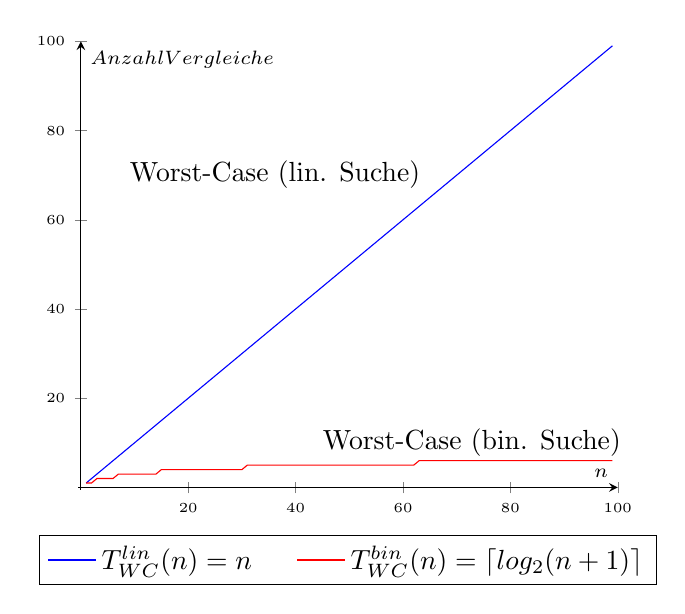
\begin{tikzpicture}
  \begin{axis}[axis lines=middle, xmin=-0.5, xmax=100, ymin=-0.5, ymax=100, xlabel=$\scriptstyle n$, ylabel=$\scriptstyle \text{Anzahl Vergleiche}$, tick label style={font=\tiny}, legend style={at={(0.5,-0.1)},anchor=north, /tikz/every even column/.append style={column sep=0.5cm}}, legend columns=-1]
    \addplot+[no marks, blue, domain=1:99, samples=99] {x};
    \addlegendentry{$T_{\text{WC}}^{\text{lin}}(n) = n$}
    \addplot+[no marks, red, domain=1:99, samples=99] {floor(ln(x+1)/ln(2))};
    \addlegendentry{$T_{\text{WC}}^{\text{bin}}(n) = \lceil log_2{(n+1)} \rceil$}
  \end{axis}
  \node at (2.5,4) {Worst-Case (lin. Suche)};
  \node at (5,0.6) {Worst-Case (bin. Suche)};
\end{tikzpicture}
\caption{Asymptotische Worst-Case-Laufzeiten im Vergleich.}
\label{figure-asymp-laufzeiten-wc-compare}
\end{figure}


Wir haben nun formal unsere Intuition bestätigt. Falls ein sortiertes Array vorliegt, können wir das Suchproblem mithilfe der binären Suche effizienter lösen als mit der linearen Suche. Falls das Array nicht sortiert ist, dann müssen wir auf die lineare Suche zurückgreifen.\autoref{table-asymp-laufzeit-bin-search} fasst die asymptotischen Laufzeiten zusammen.

\begin{table}[htb]
\centering
\begin{tabular}{|c|c|c|c|}
\hline
Algorithmus & Best-Case & Average-Case & Worst-Case \\ \hline
Binäre Suche & $1$ & $\approx log_2{(n)}$ & $\lceil log_2{(n+1)} \rceil$ \\ \hline
\end{tabular}
\caption{Asymptotische Laufzeiten für die binäre Suche mit $n$ Elementen. Die Analyse für den Average-Case ist sehr aufwendig und wird hier nicht betrachtet.}
\label{table-asymp-laufzeit-bin-search}
\end{table}
